\section{¿Qué es la tolerancia a fallas?}
\begin{frame}
	\frametitle{¿Qué es la tolerancia a fallas?}
	\begin{columns}[T]
		\begin{column}{.5\textwidth}
			\centering
			Ariane 5 - 1996
			\vfill
			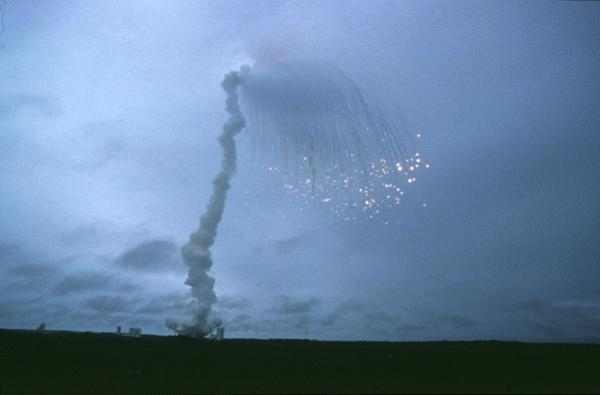
\includegraphics[scale=1]{images/ariane5.jpg}
		\end{column}
		\begin{column}{.5\textwidth}
			\centering
			Schiaparelli - 2016
			\vfill
			
\includegraphics[scale=0.2]{images/mars.jpg}
		\end{column}
	\end{columns}    
\end{frame}

\subsection{Atributos de la fiabilidad}
\begin{frame}
	\frametitle{Confiabilidad}
	Es la probabilidad de que un sistema continúe operando correctamente durante un intervalo de tiempo dado. 
	“Es la capacidad del sistema o componente de realizar sus funciones requeridos bajo las condiciones establecidas durante un período de tiempo específico” (IEEE)
	\LARGE
	$$
	R(t) = e^{-\lambda t }
	$$
\end{frame}

\begin{frame}
	\frametitle{Disponibilidad}
	Es la probabilidad de que el sistema esté operando correctamente en un determinado instante de tiempo. 
	\LARGE
	$$
	A(t) = 1/T \int_0^T{A(t) dt}
	$$
\end{frame}

\begin{frame}
	\frametitle{Seguridad}
	Se considera como una extensión de la confiabilidad. Se define como la probabilidad de que el sistema sea capaz de realizar sus funciones correctamente o continuar sus funciones en una manera a prueba de fallas. 
\end{frame}

\subsection{Falla, Error, Avería}
\begin{frame}[c]
	\begin{center}
		\LARGE
		\textbf{Falla \textrightarrow Error \textrightarrow Avería}\\
		\textit{Fault \textrightarrow Error \textrightarrow Failure}
	\end{center}
\end{frame}
